\subsection{Level3.3: 任意の評価用データを用いた評価}
\subsubsection{アプローチ}
学習時のデータ(教師データ)との違いが少ないほど認識率が高く、逆に教師データとの違いが多いほど認識率が低くなるとの仮定のもと、以下に示す評価用データを用意した。\\
今回は違いを分かり易くするため、0と1で表現された教師用データから、1の位置をズラす範囲とその数によって違いを作っている。つまり、より多くの1がより大きくズレていれば、より違いが多いということである。
\begin{figure}[htbp]
  \begin{center}
    \begin{tabular}{c}

      % 1
      \begin{minipage}{0.33\hsize}
        \begin{center}
          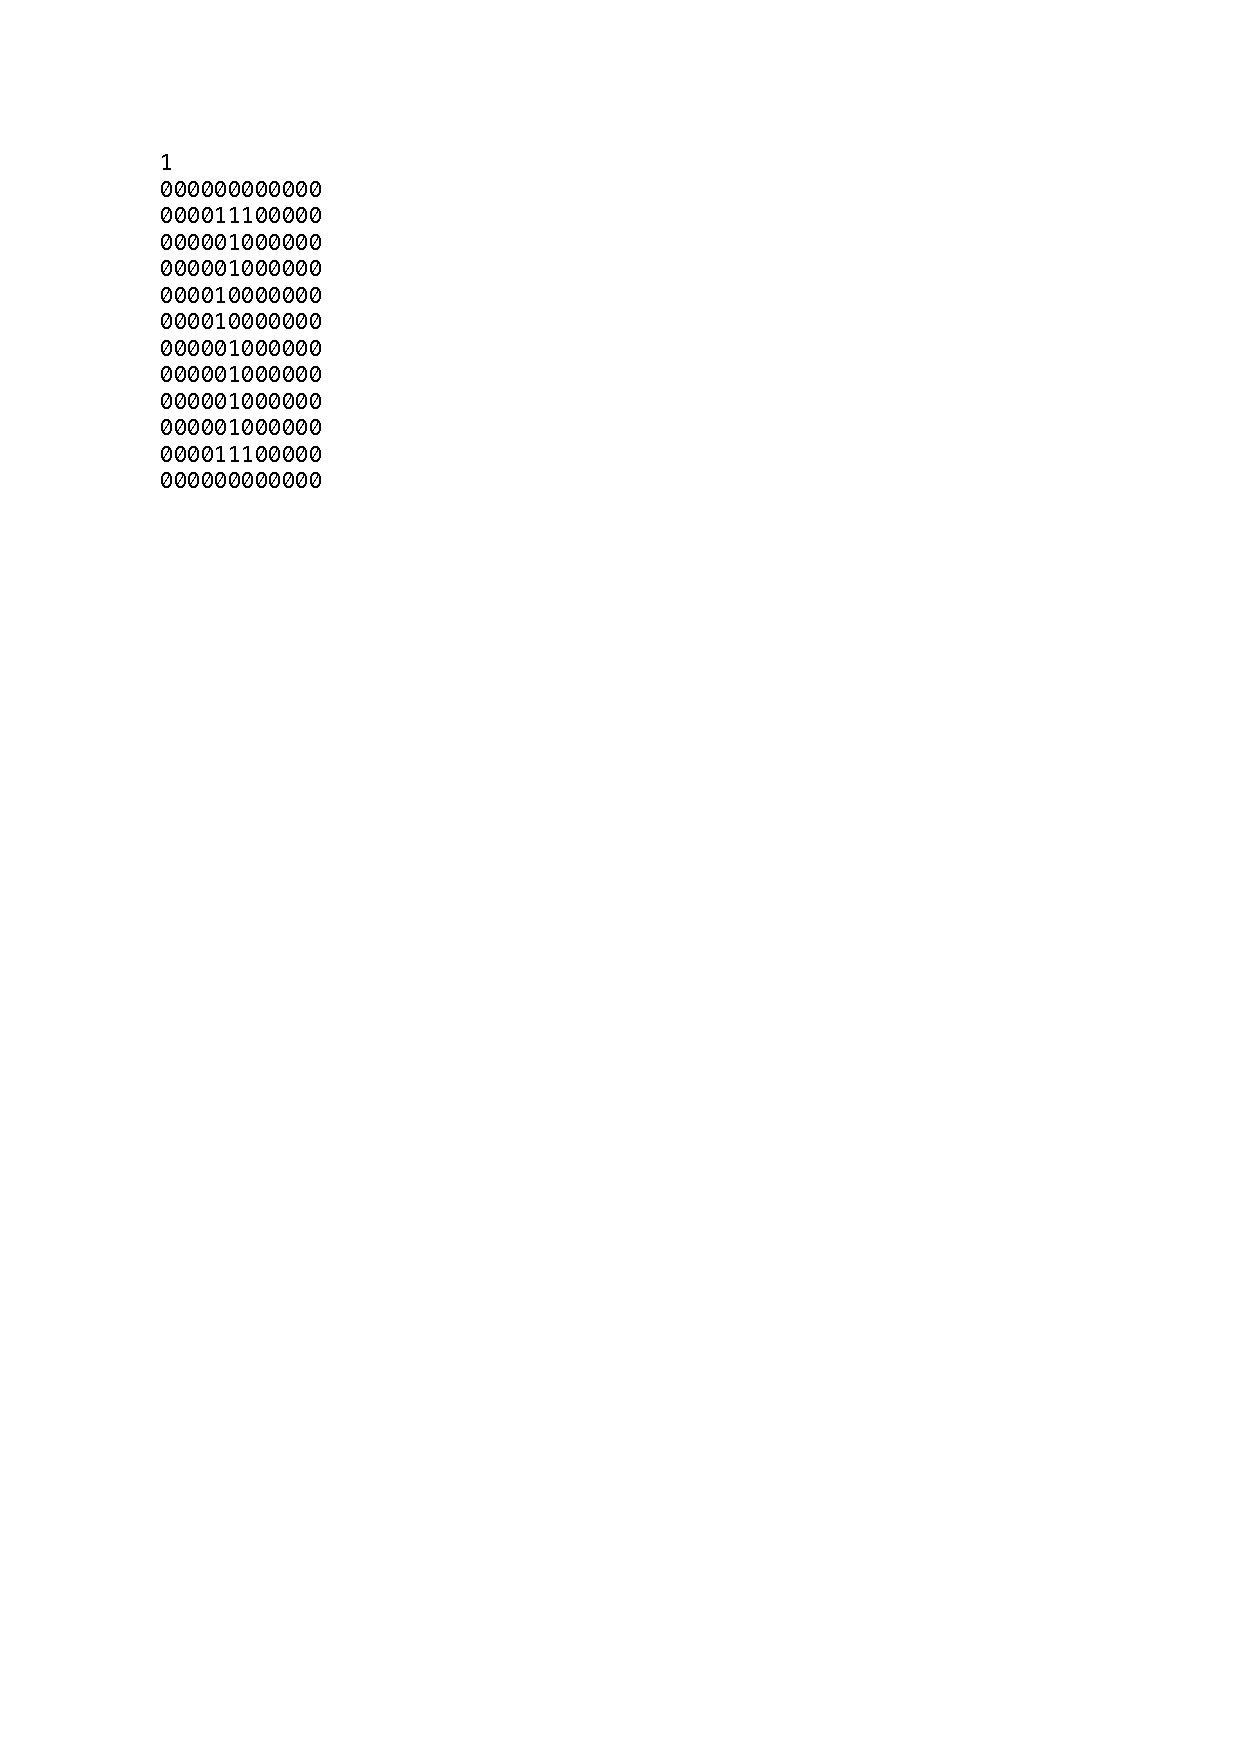
\includegraphics[clip, width=3.2cm]{./lebel3-3figs/eva1-3.pdf}
          \hspace{2.3cm} (1)違いが1番少ないデータ
        \end{center}
      \end{minipage}

      % 2
      \begin{minipage}{0.33\hsize}
        \begin{center}
          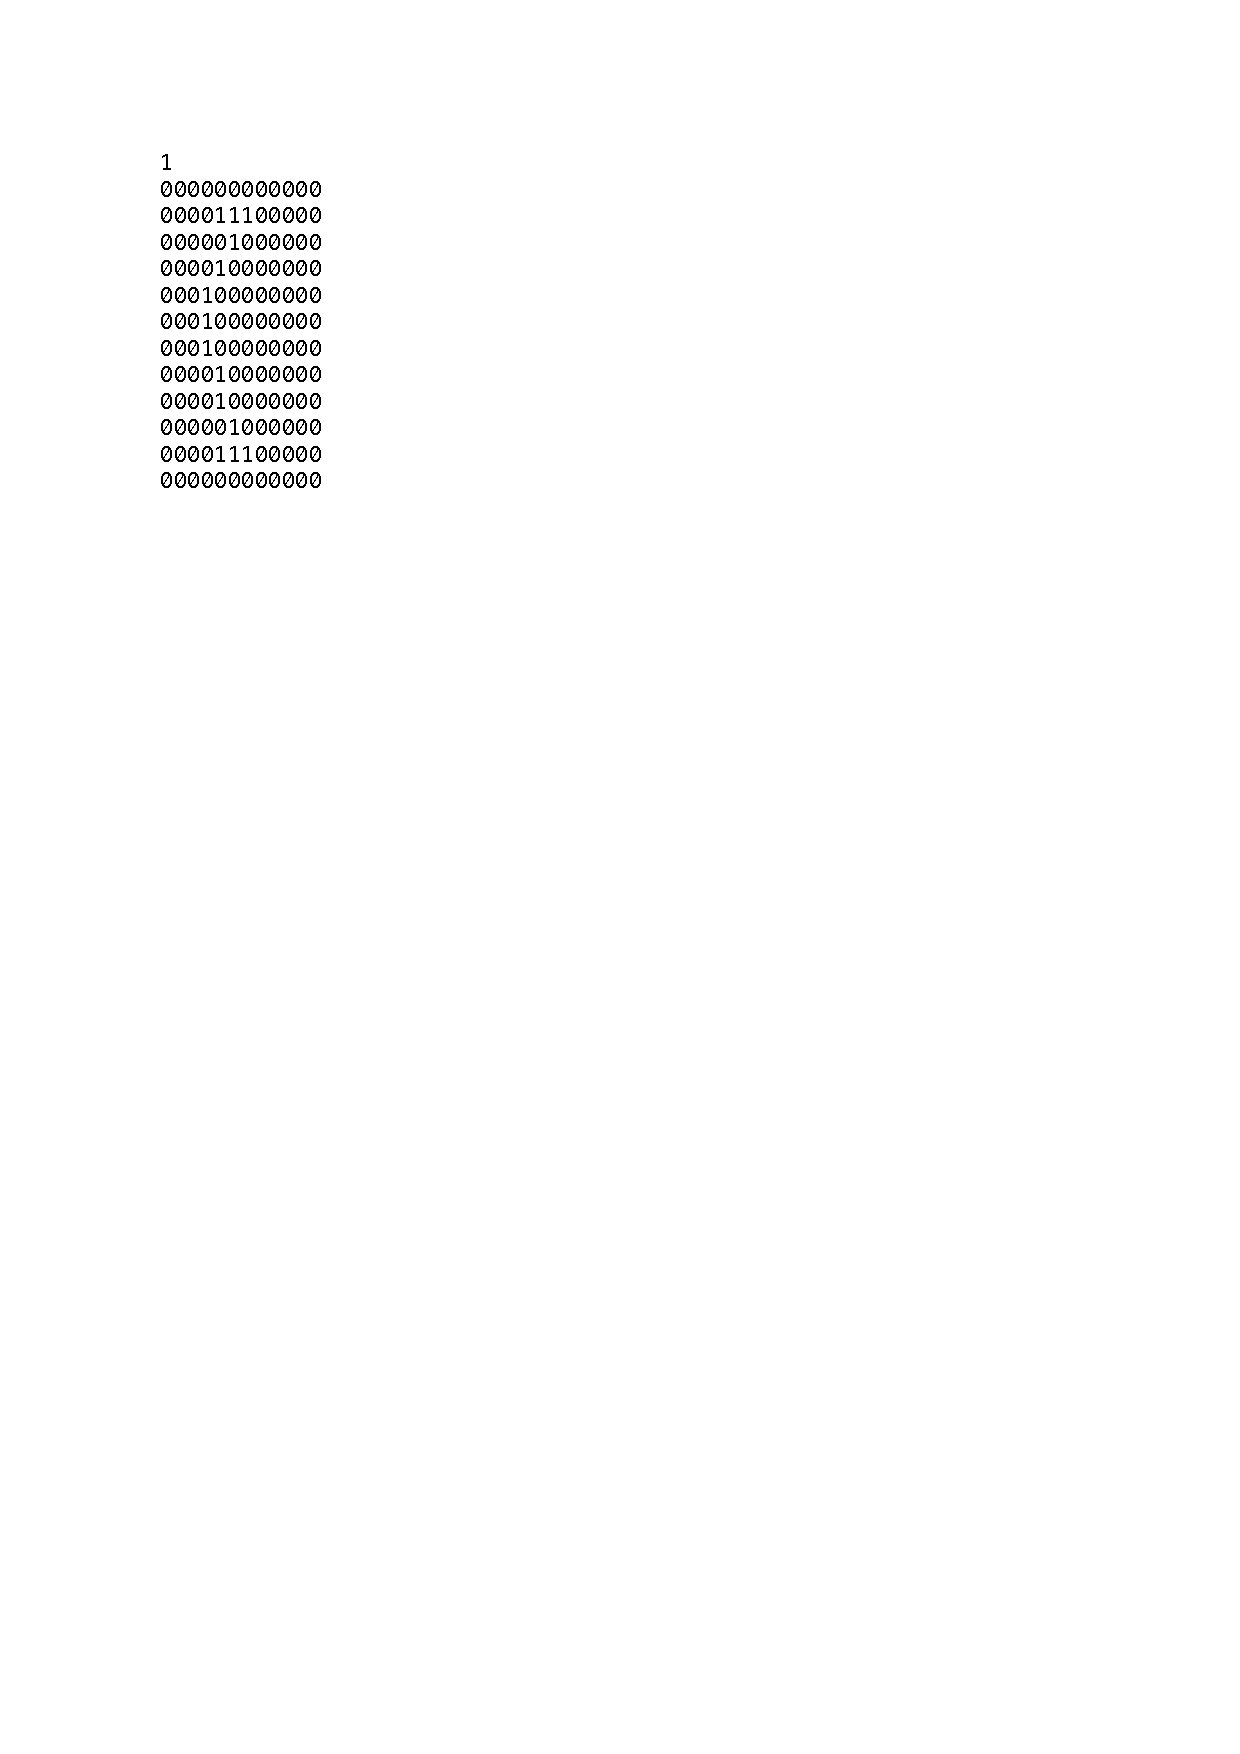
\includegraphics[clip, width=3.2cm]{./lebel3-3figs/eva1-4.pdf}
          \hspace{2.3cm} (2)違いが2番目に少ないデータ
        \end{center}
      \end{minipage}

      % 3
      \begin{minipage}{0.33\hsize}
        \begin{center}
          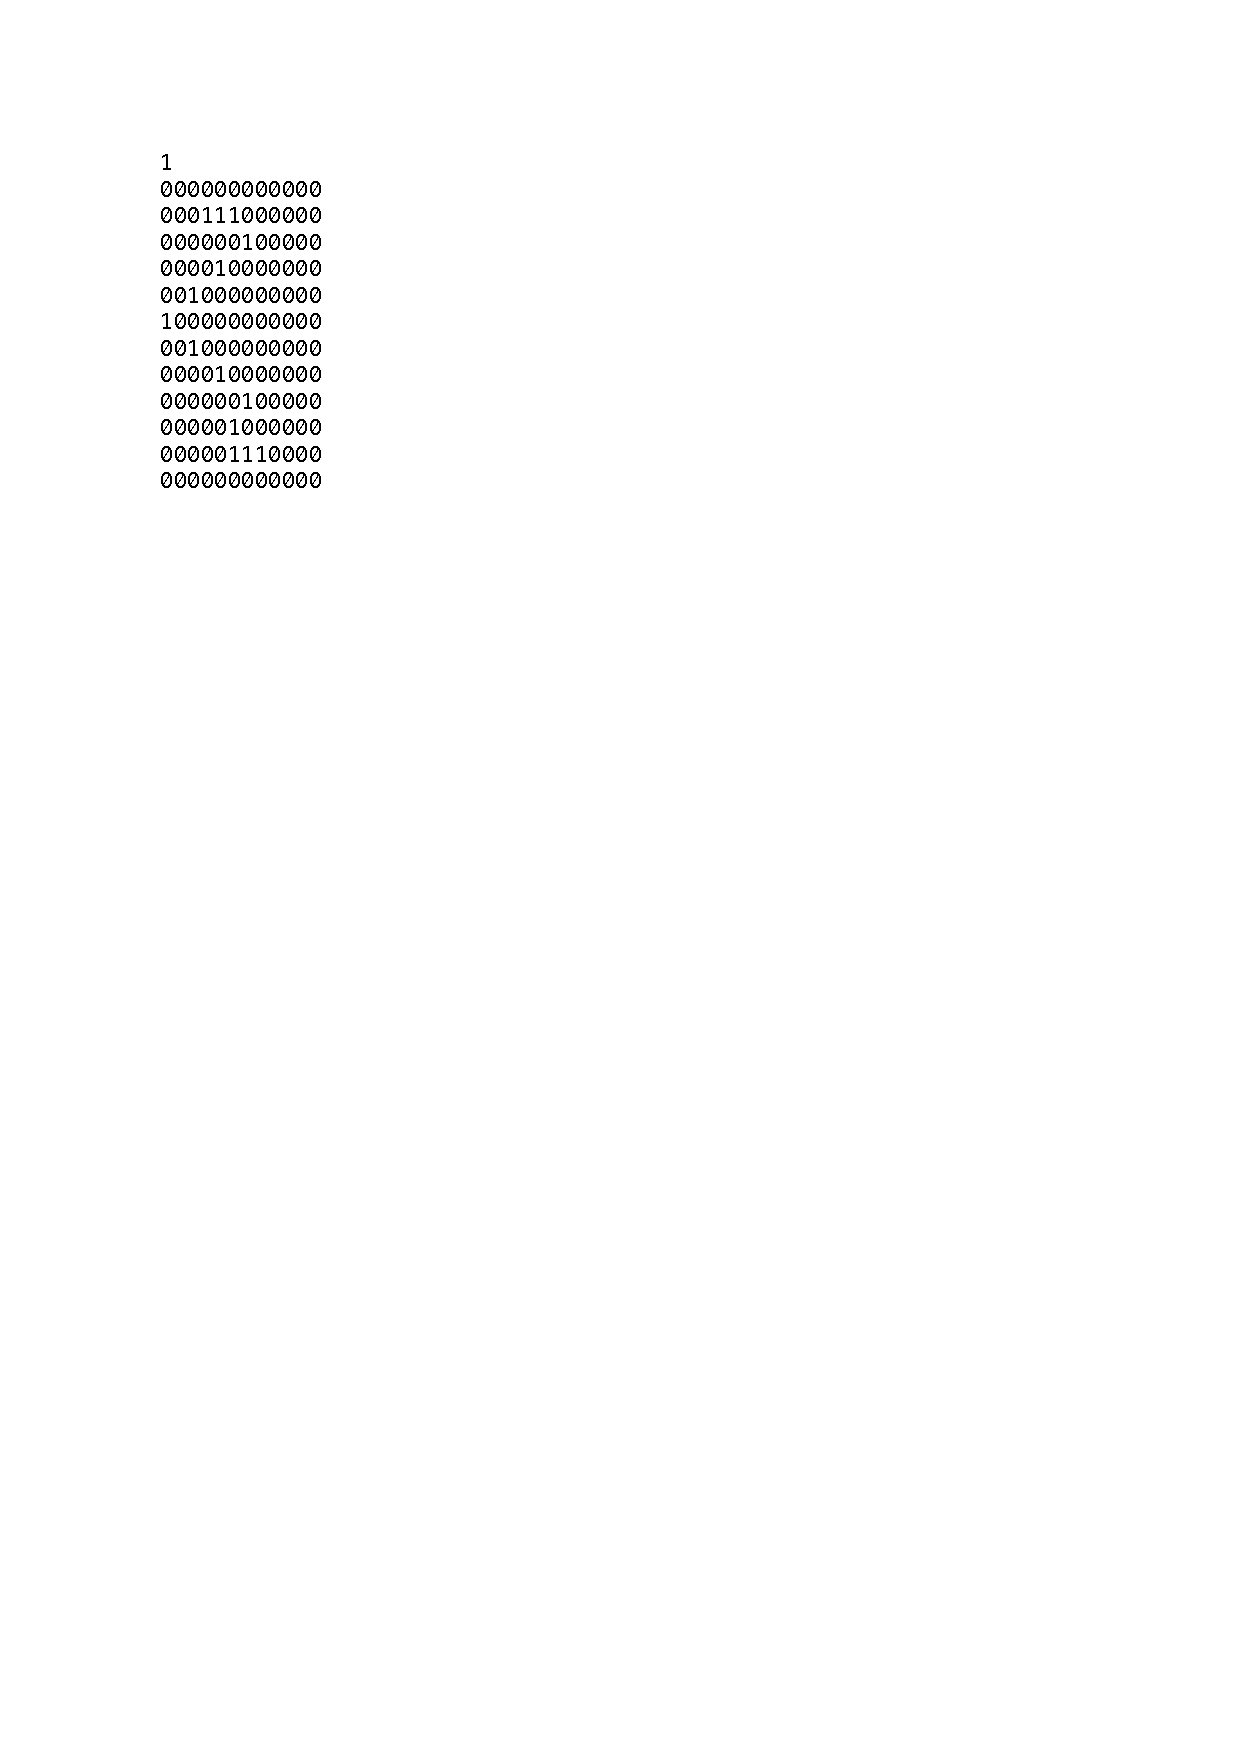
\includegraphics[clip, width=3.2cm]{./lebel3-3figs/eva1-5.pdf}
          \hspace{2.3cm} (3)違いが最も多いデータ
        \end{center}
      \end{minipage}

    \end{tabular}
    \caption{任意の評価用データ}
  \end{center}
\end{figure}

\subsubsection{結果}
最初に「1」という文字を学習させた。学習したことによる学習度合いを図6に示す。\\
\begin{figure}[htbp]
  \begin{center}
    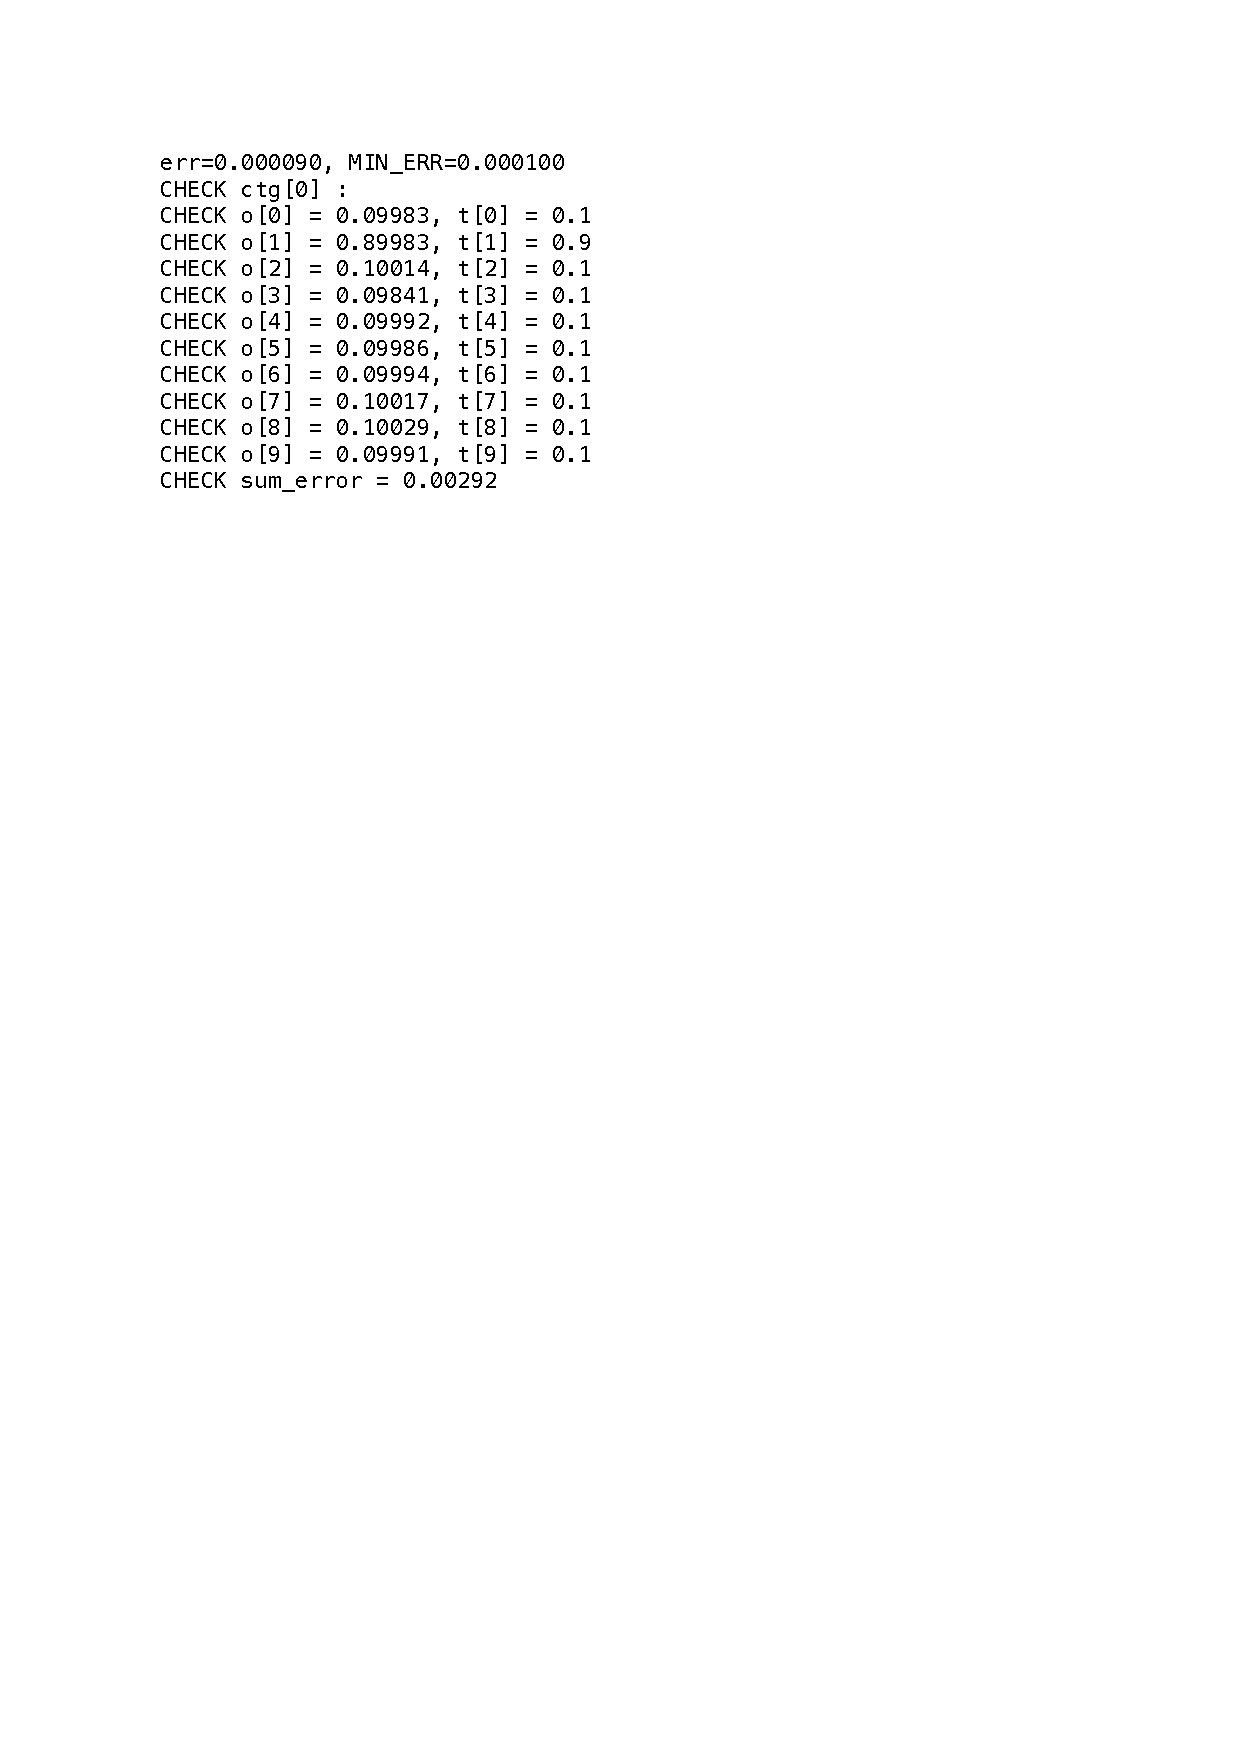
\includegraphics[clip,width=5.5cm]{./lebel3-3figs/c.pdf}
    \caption{学習事例に対する学習度合いを確認}
  \end{center}
\end{figure}
\\用意した任意の評価用データに対する適応度合いを確認する。
\begin{figure}[htbp]
  \begin{center}
    \begin{tabular}{c}

      % 1
      \begin{minipage}{0.33\hsize}
        \begin{center}
          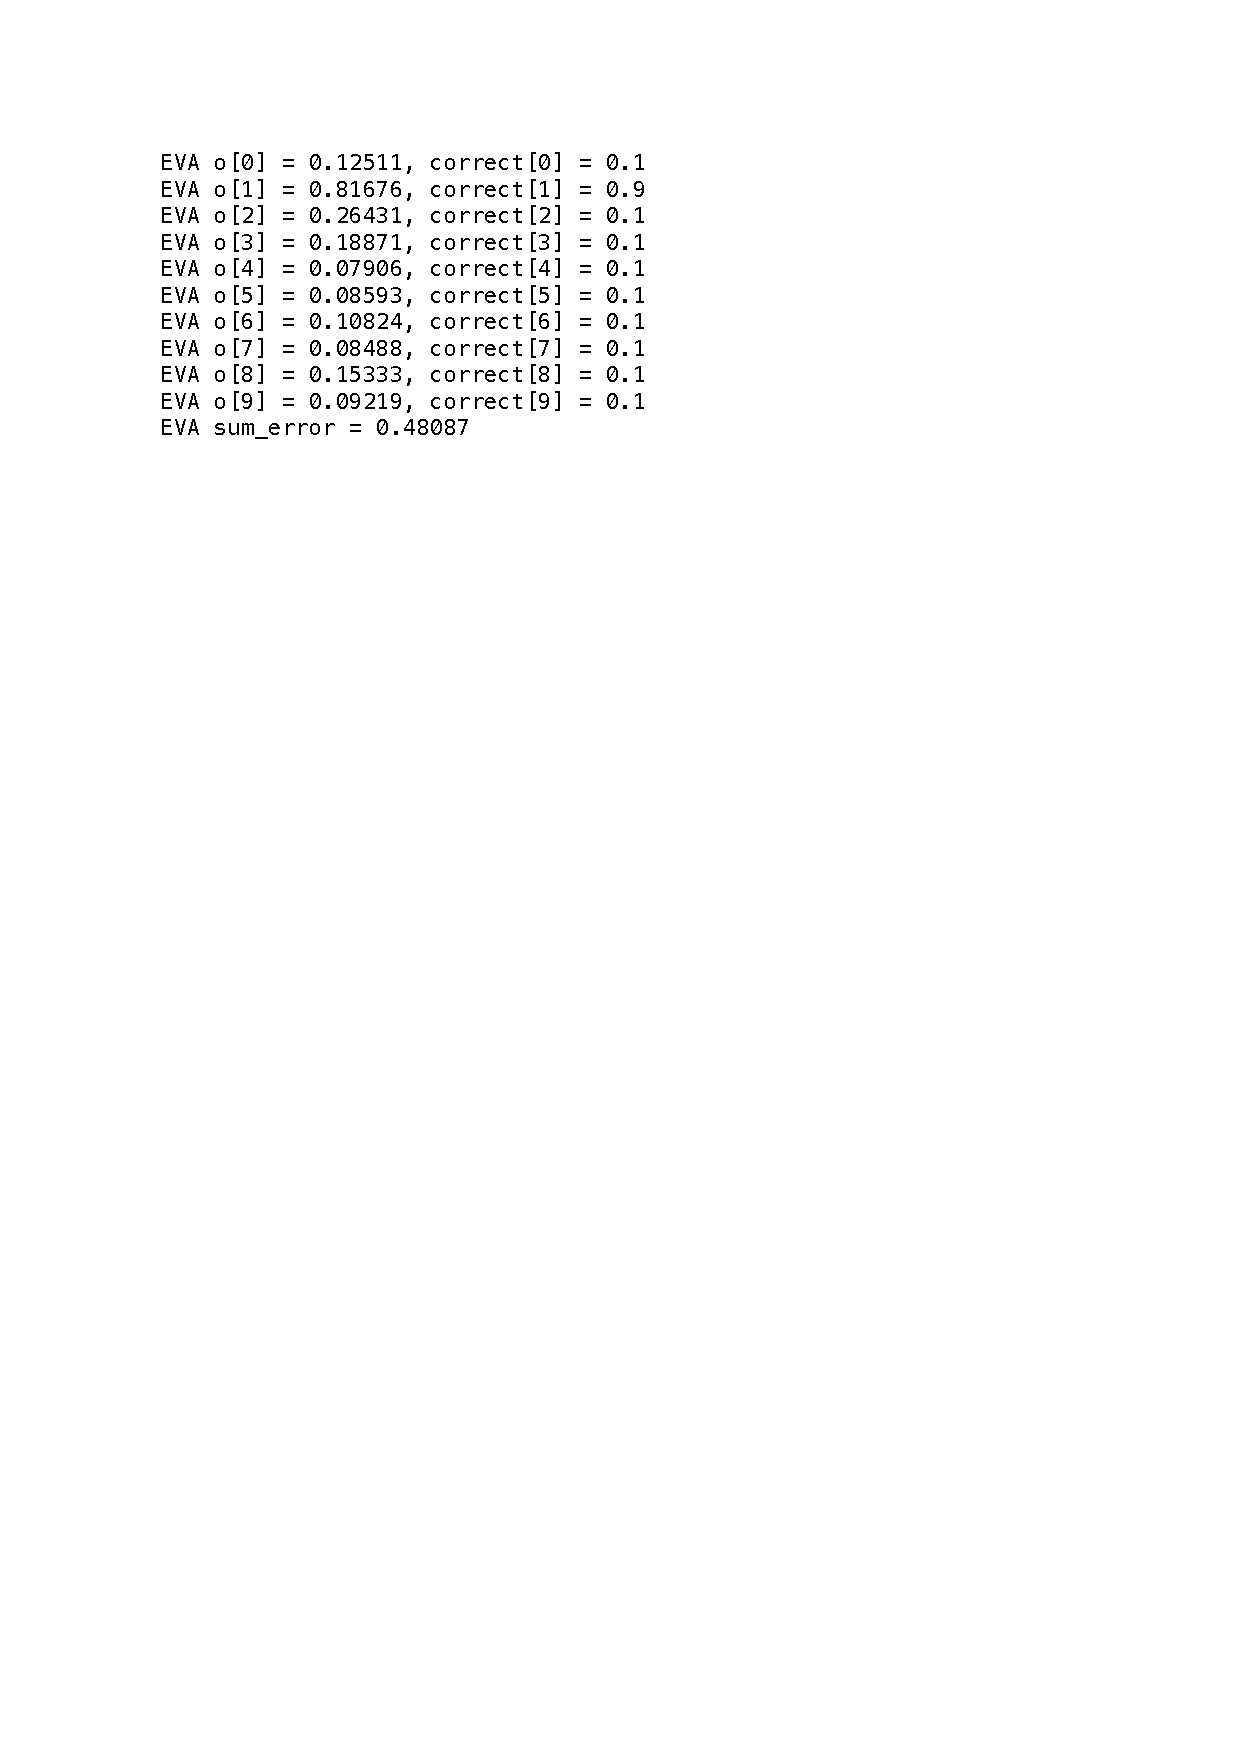
\includegraphics[clip, width=5.0cm]{./lebel3-3figs/e1.pdf}
          \hspace{2.3cm} (1)違いが1番少ないデータ
        \end{center}
      \end{minipage}

      % 2
      \begin{minipage}{0.33\hsize}
        \begin{center}
          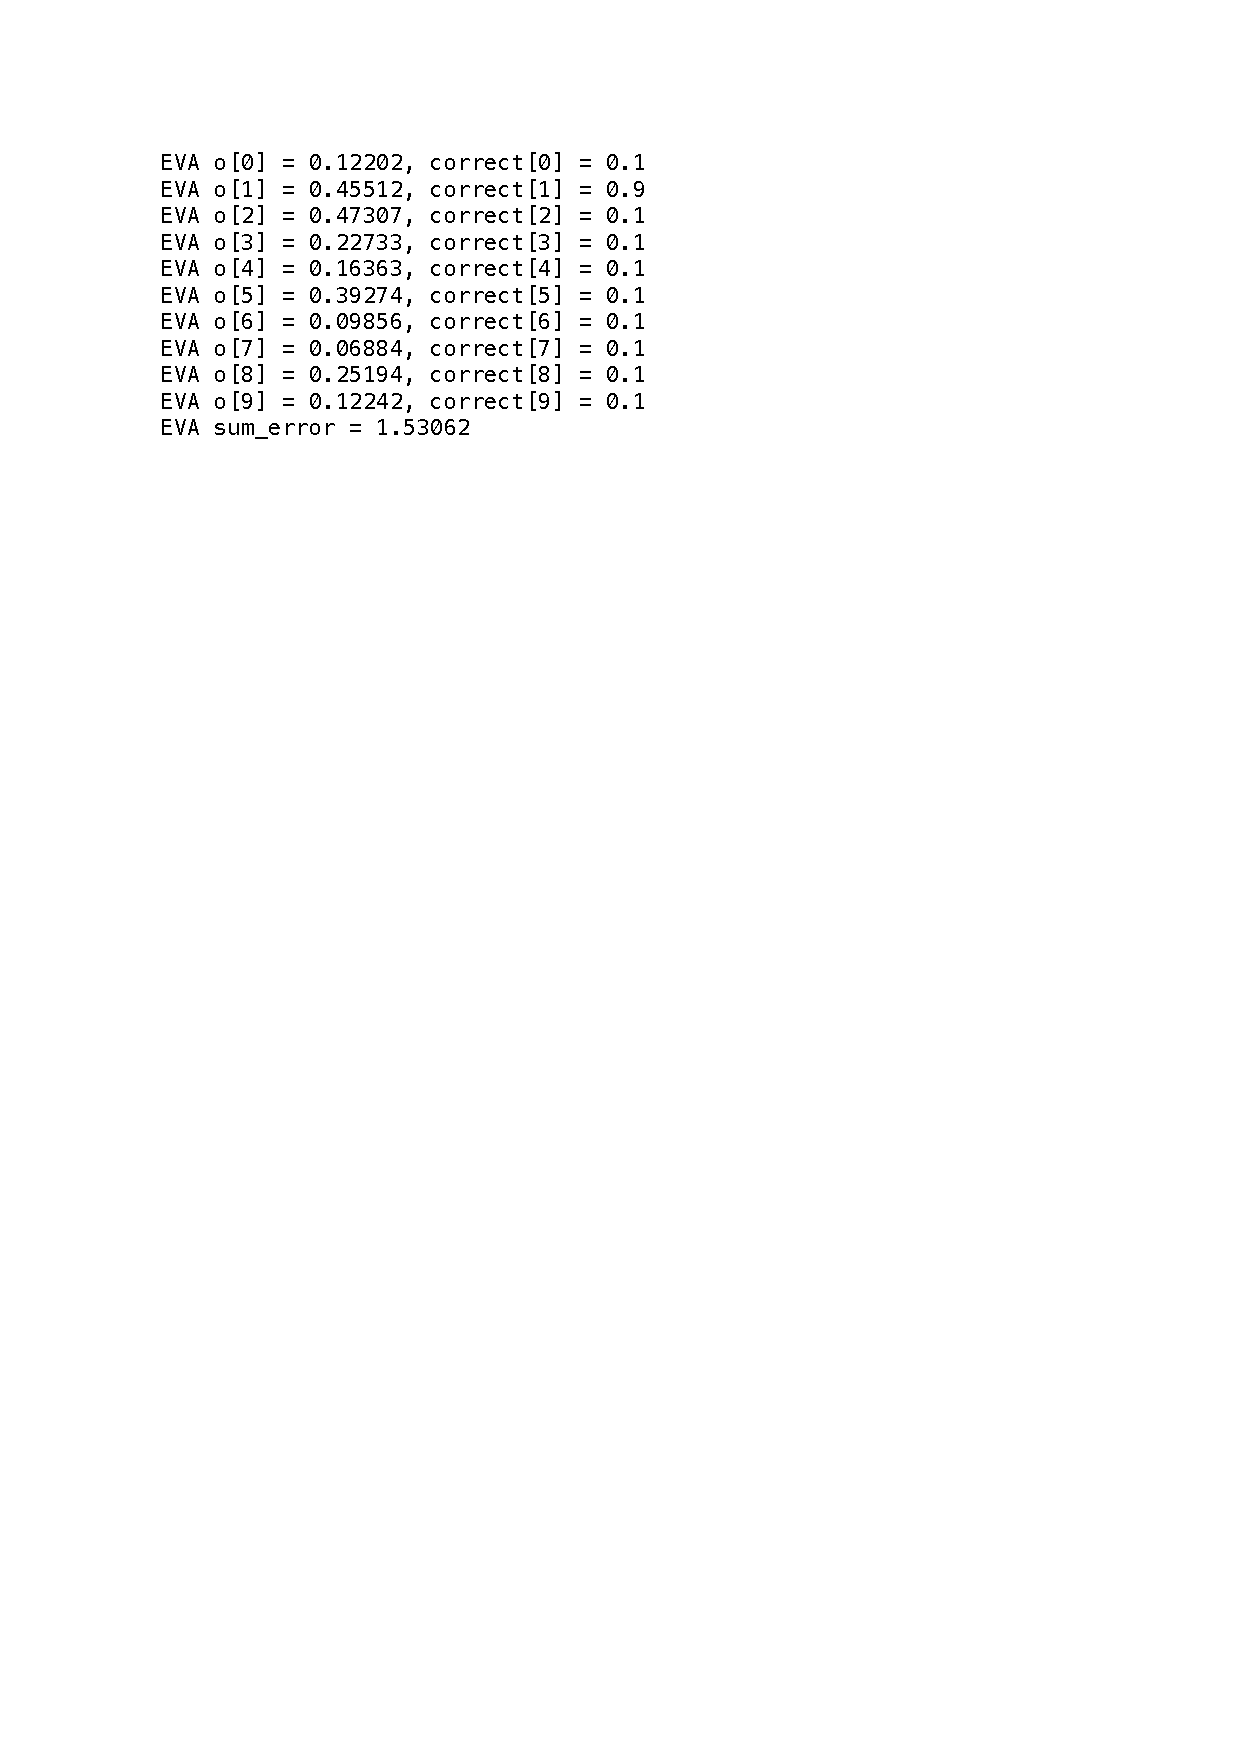
\includegraphics[clip, width=5.0cm]{./lebel3-3figs/e2.pdf}
          \hspace{2.3cm} (2)違いが2番目に少ないデータ
        \end{center}
      \end{minipage}

      % 3
      \begin{minipage}{0.33\hsize}
        \begin{center}
          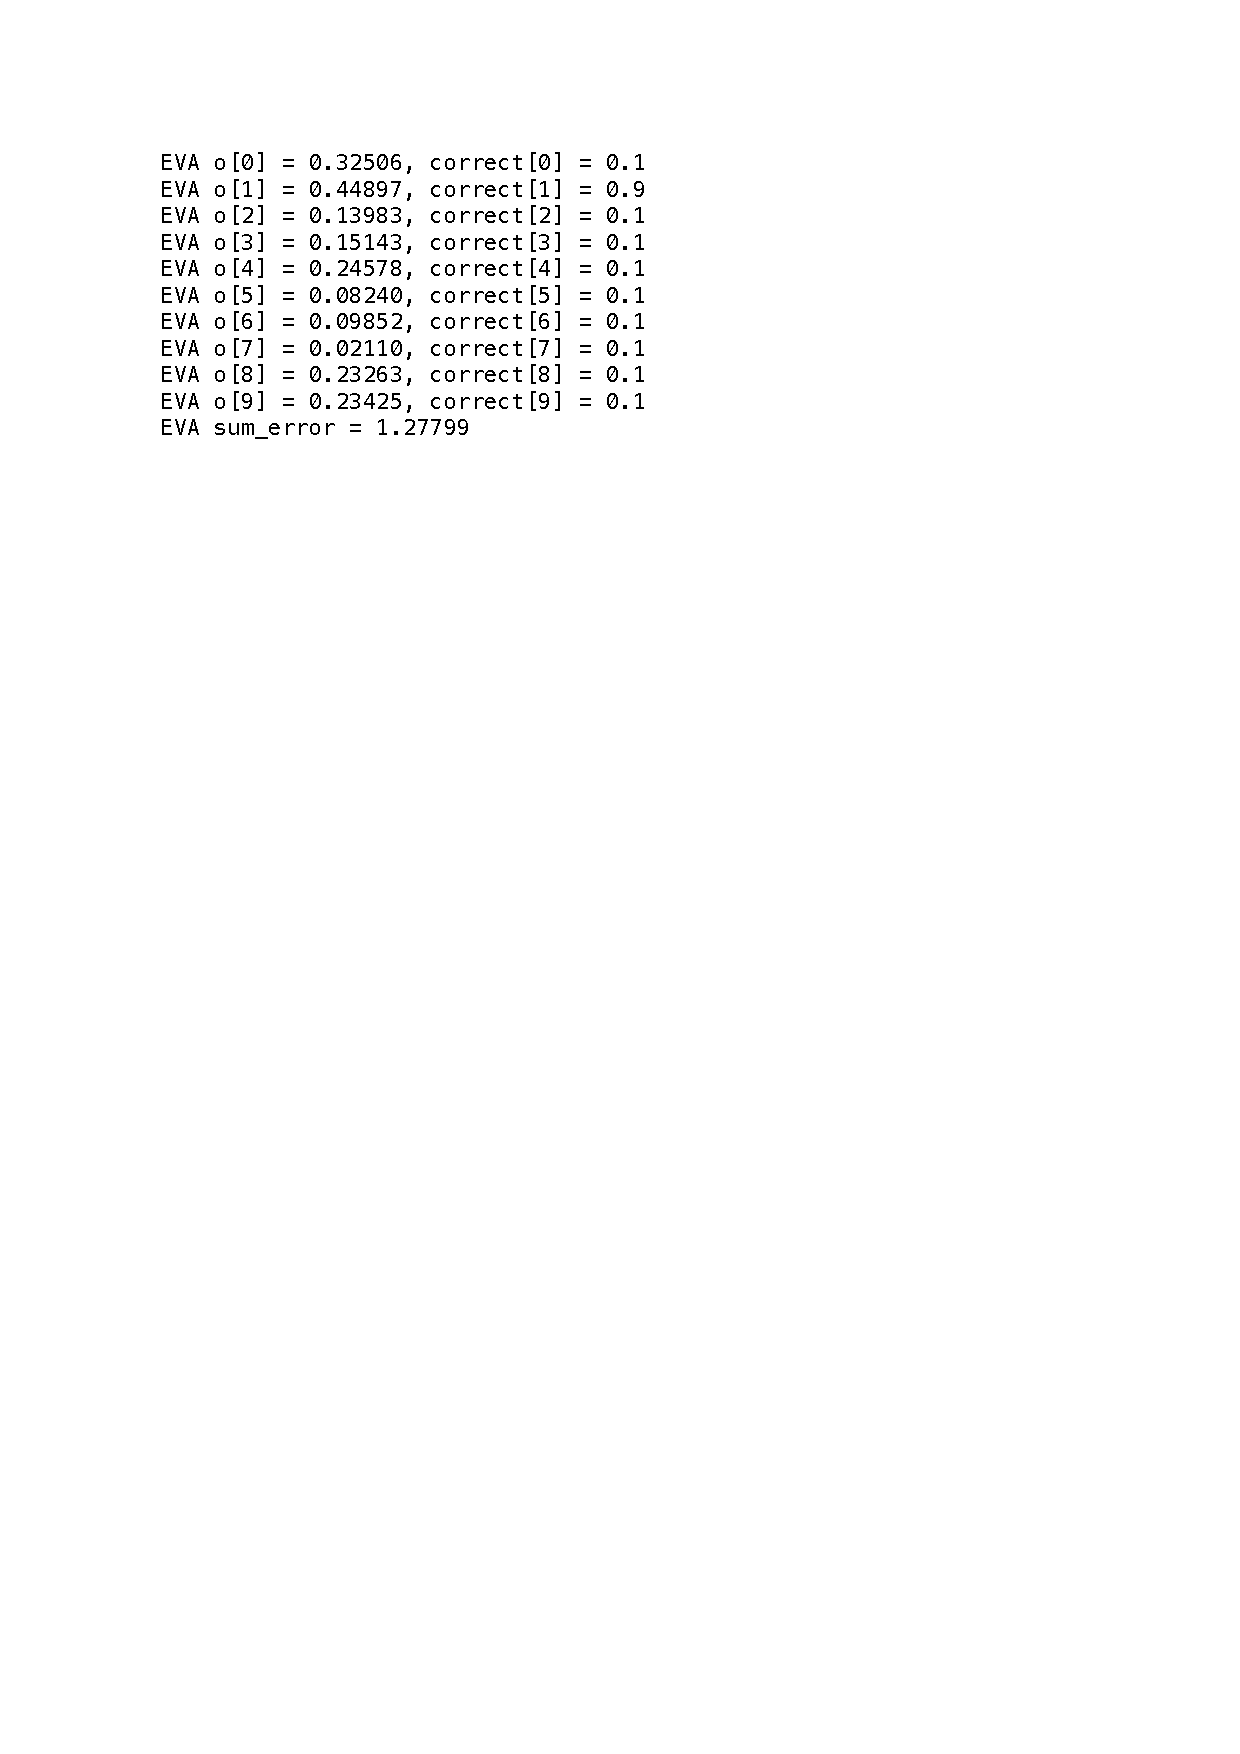
\includegraphics[clip, width=5.0cm]{./lebel3-3figs/e3.pdf}
          \hspace{2.3cm} (3)違いが最も多いデータ
        \end{center}
      \end{minipage}

    \end{tabular}
    \caption{任意の評価用データ}
  \end{center}
\end{figure}
\subsubsection{考察}
上記の結果で注目すべきはEVAo[1]という項目であり、この値が0.9に近ければ近いほど、より「1」と認識された事を表している。違いが多いほどこの値が小さくなり、「1」と認識されにくいことが分かる。\\
したがって、仮説通り教師データとの違いが少ないほど認識率が高く、逆に教師データとの違いが多いほど認識率が低いといえる。\\ところで、違いが2番目に少ないデータと1番多いデータの認識率はあまり変わらない。
教師データに用いられた「1」を表現する0と1の羅列を「1」という形を保ったまま、重なるところがないようにズラしたところ、認識率は0.03以下になった。一方で、「1」の上端下端のみにしたところ認識率は0.6以上になった。もちろん認識率0.6では「1」と呼べないが、「1」と認識できるデータよりも認識率が大きいため、教師データに対してより重なる部分が多ければ、認識され易いと考えることが出来る。

